\chapter{Инструменты и оборудование}


\section{Паяльное оборудование}

\subsection{Паяльник}

Паяльник\ --- обязателен дешевый сетевой мощностью не менее 20\,Вт, типа
ЭПСН-25/220. Ограничитель мощности или регулятор температуры легко собрать
самостоятельно.

Для сборки электроники хорошо также иметь маленький монтажный 12\,В 8\,Вт от
паяльной станции ZD-927 ($\sim$100\,р), без самой станции. Если не жалко 500\,р,
берите станцию ZD-927 целиком, внутри простейший регулятор мощности, и вам не
понадобится источник питания на 12\,В, который вы еще не сделали.

\noindent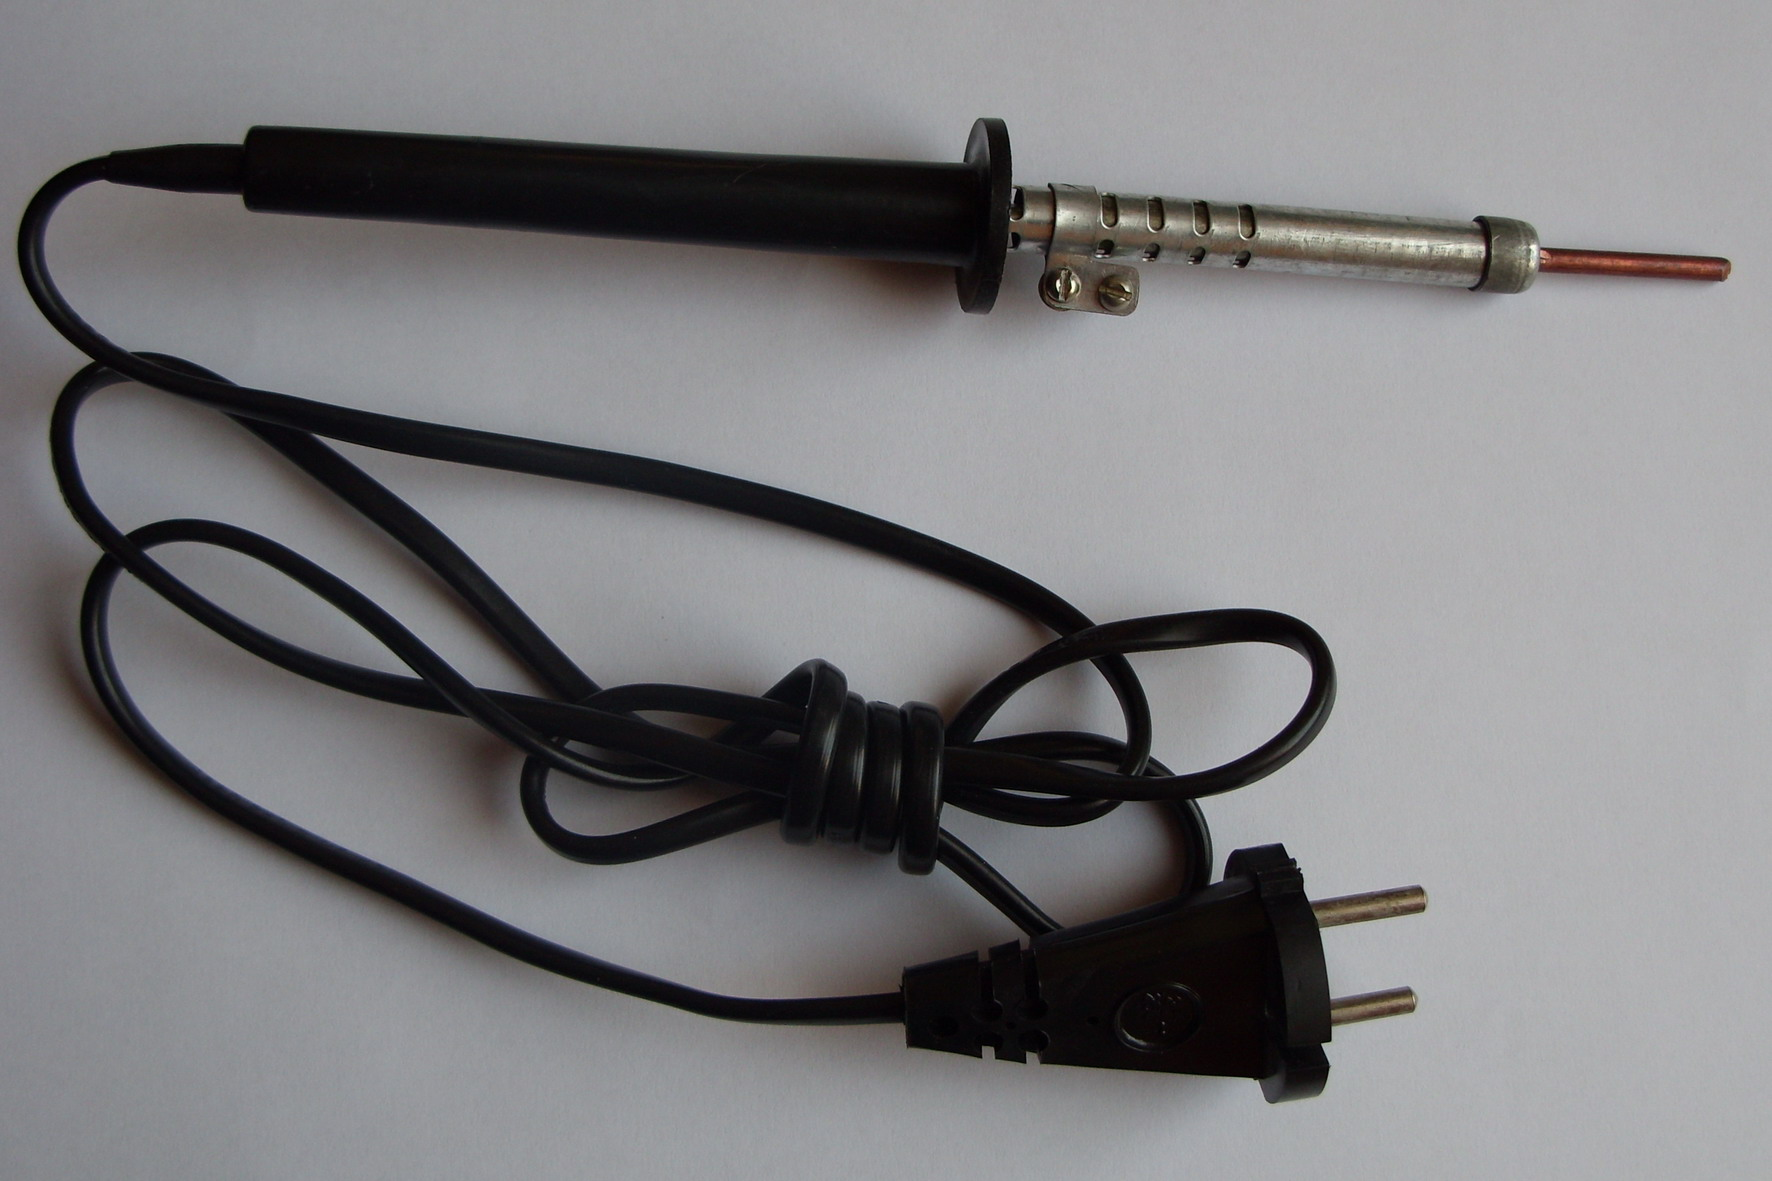
\includegraphics[width=0.4\textwidth]{tech/tools/solder/EPSN25.jpg}
\textbf{Паяльник ЭПСН-25/220}

\noindent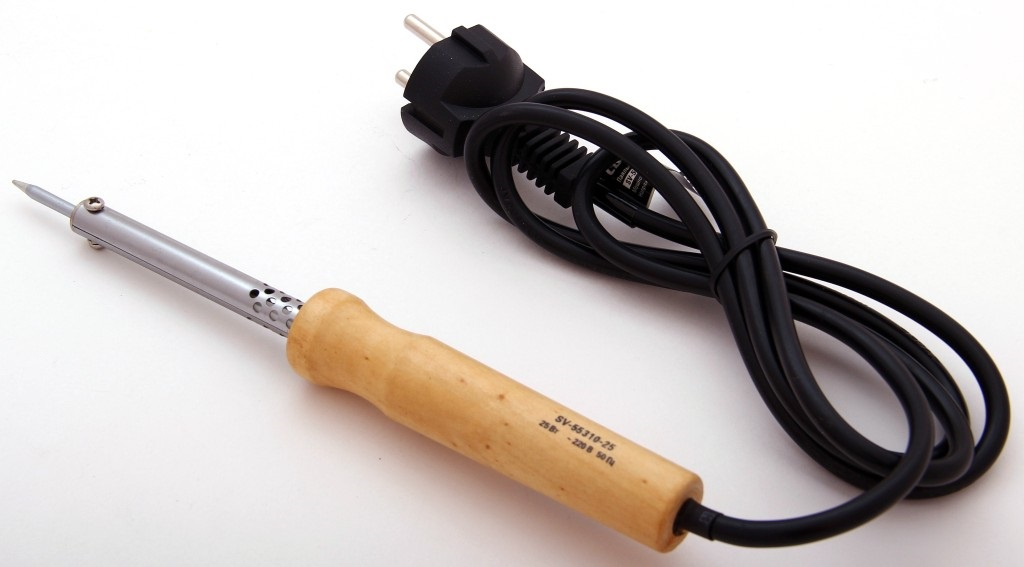
\includegraphics[width=0.4\textwidth]{tech/tools/solder/SV-55310-25.jpg}
\textbf{Паяльник 220В 25Вт, СВЕТОЗАР, SV-55310-25 230\,р.}

\noindent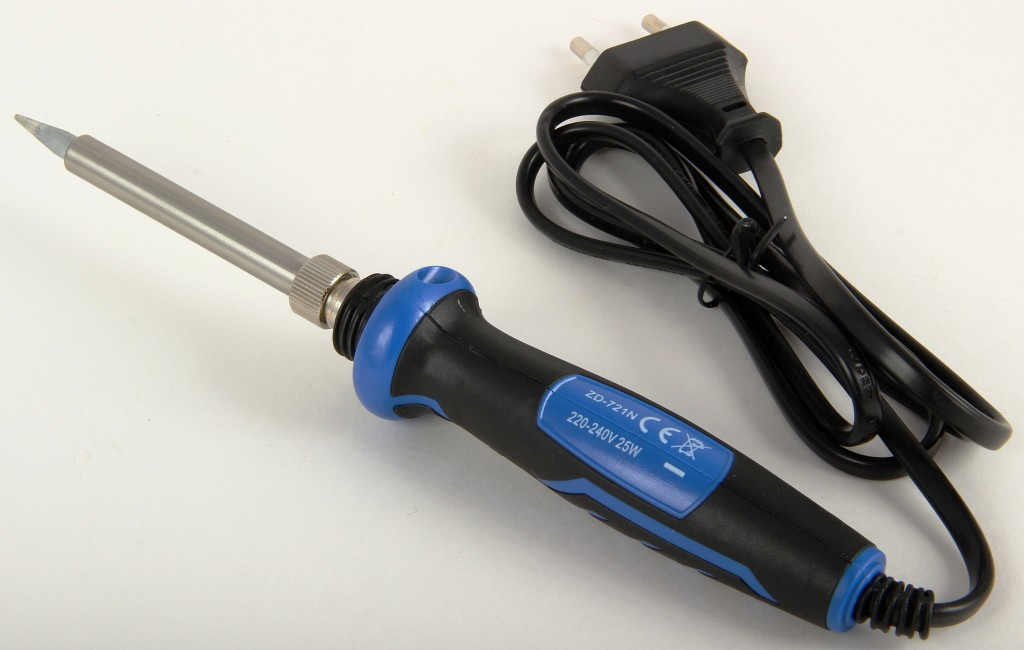
\includegraphics[width=0.4\textwidth]{tech/tools/solder/ZD-721N.jpg}
\textbf{Паяльник 220В 25Вт ZD-721N 175\,р.}

\noindent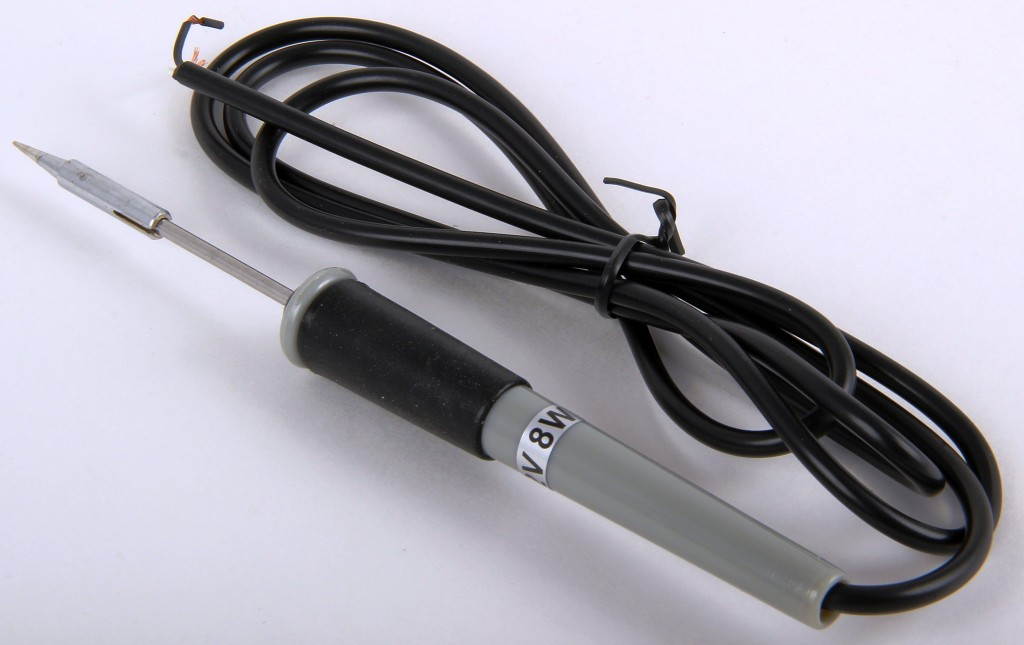
\includegraphics[width=0.4\textwidth]{tech/tools/solder/Iron8W.jpg}
\textbf{Паяльник для станции ZD-927 12\,В 8\,Вт 85\,р.}

\subsection{Паяльная станция}

Из всего разнообразия для хоббита оптимальным являются паяльные станции Lukey
702/853D (3000+\,р). Для работы или регулярного хобби паяльная станция с феном,
а может даже и встроенным источником питания, вещь незаменимая, и не такая уж
дорогая.

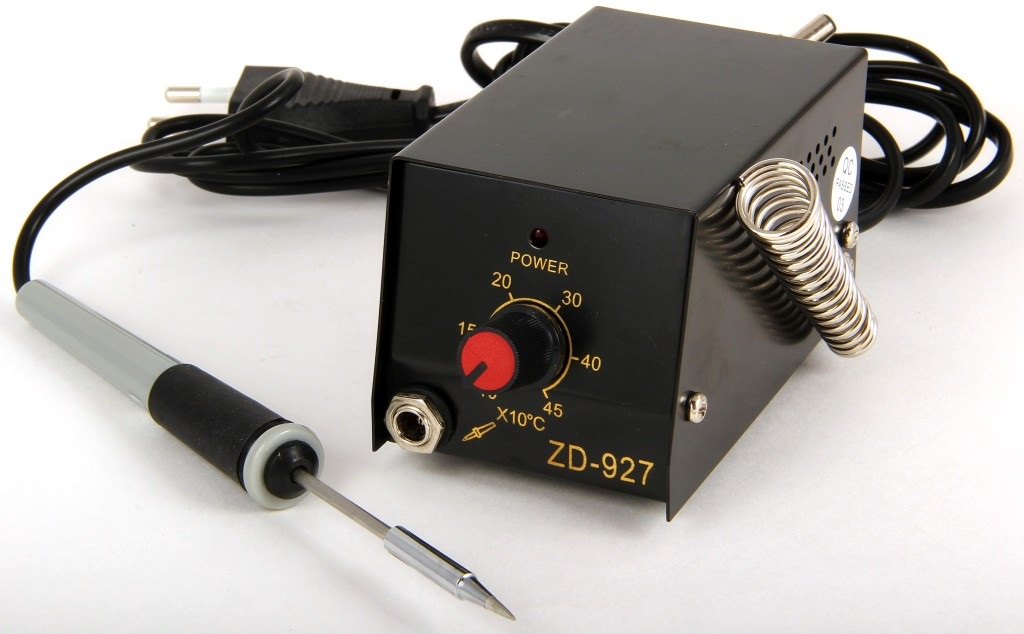
\includegraphics[width=0.45\textwidth]{tech/tools/solder/ZD927.jpg}
\textbf{Паяльная станция ZD-927 520\,р.}

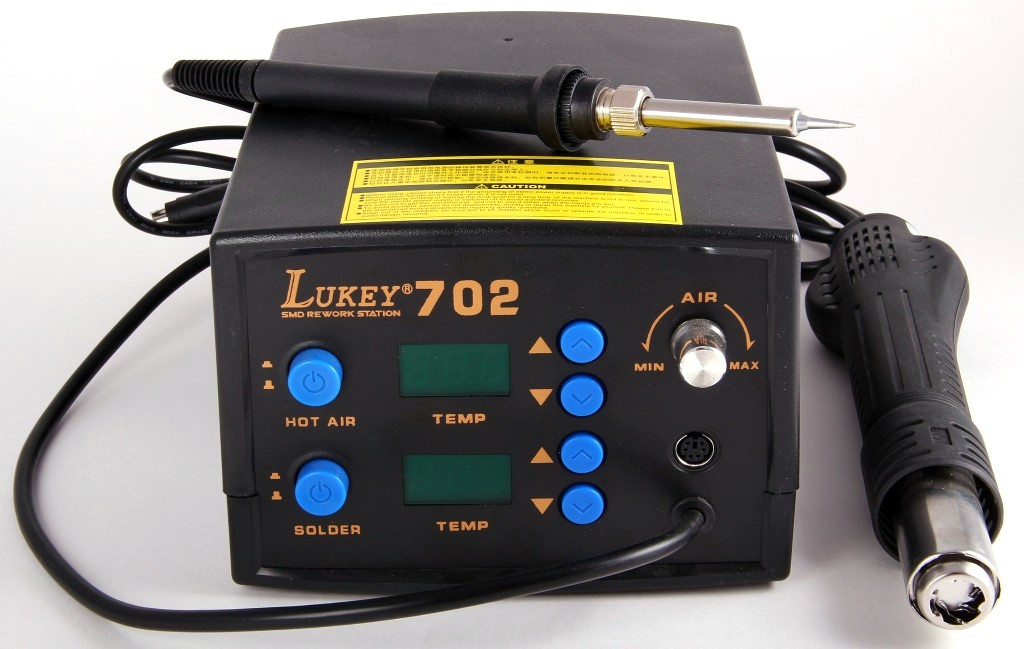
\includegraphics[width=0.45\textwidth]{tech/tools/solder/Lukey702.jpg}
\textbf{Паяльная станция LUKEY 702 3100\,р.}

\clearpage
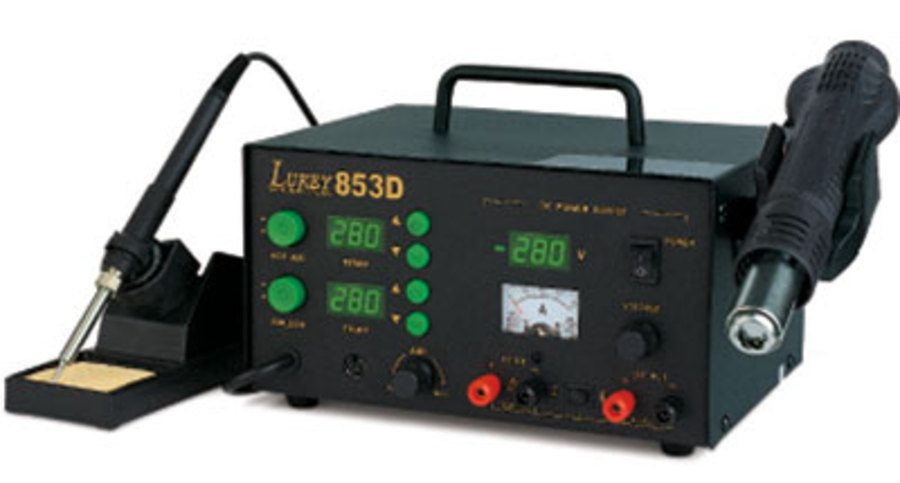
\includegraphics[width=0.95\textwidth]{tech/tools/solder/Lukey853D.jpg}

\textbf{Паяльная станция LUKEY 853D с источником питания 5200\,р.}
\clearpage



\section{JTAG-адаптер}

% \input{jtag/soft}
% \input{stlink/stlink1}

\section{Отладочные платы}

Прежде чем начать работать с отдельными \mk, устанавливая их на плату
собственной разработки, для быстрого старта используют \term{отладочные
платы}\note{development board, demo board}

\subsection{Arduino /Atmel Mega AVR8/}

\subsection{Cortex-Mx} %См. \ref{devkitcmx}

\subsection{CubieBoard /Cortex-A8 AllWinner A10/}

\subsection{Raspberry Pi /ARM11 BCM3032/}

\subsection{BlackSwift /MIPS/}

\subsection{VoCore /MIPS/}

\secrel{Радиомонтажный инструмент}\secdown

Пара надфилей, заточной камень на дрель, комплект сверел и несколько листов
наждачки.

\secrel{Pro'sKit}
Отдельного обзора заслуживает инструмент и наборы Pro'sKit
% \href{http://www.proskit.com/}{ProsKit}
%  / \href{http://www.proskit.msk.ru/index.html}{ru}.

\clearpage
\noindent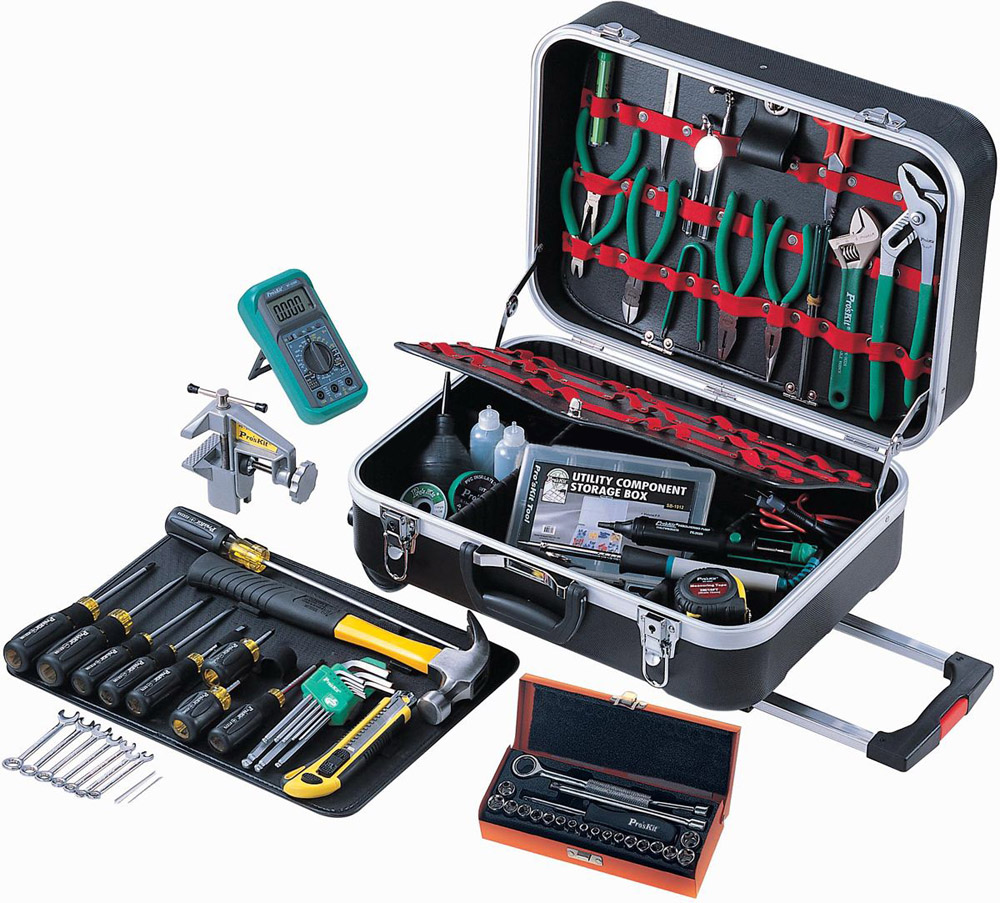
\includegraphics[height=0.95\textheight]{tech/tools/proskit/PK5308BM.jpg}

\textbf{PK-5308BM универсальный набор инструментов}

\clearpage
\noindent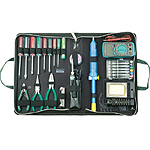
\includegraphics[height=0.95\textheight]{tech/tools/proskit/1PK-616B.jpg}

\textbf{1PK-616B Набор инструментов для электроники профессиональный}

\clearpage\label{1PK-813B}
\noindent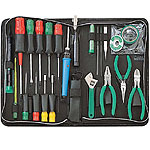
\includegraphics[height=0.95\textheight]{tech/tools/proskit/1PK-813B.jpg}

\textbf{1PK-813B Набор базовых инструментов для электроники}

\clearpage

По личному опыту: в 1PK-813B не хватает

\begin{itemize}
  \item мелкого мультиметра,
  \item стриппера 1PK-3001E,
  \item микрокусачек типа 8PK-30D,
  \item канифоли,
  \item ножа,
  \item настроечную отвертку заменить индикаторной.
\end{itemize}

\clearpage
\secrel{Инструмент до 1000\,В}

Для электромонтажных работ обязательно приобретите комплект
высоковольтного инструмента до 1000\,В:

\begin{tabular}{p{0.45\textwidth} p{0.45\textwidth}}
\noindent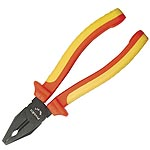
\includegraphics[width=0.45\textwidth]{tech/tools/proskit/PM-911.jpg}
&
\noindent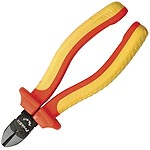
\includegraphics[width=0.35\textwidth]{tech/tools/proskit/PM-917.jpg}
\\

\textbf{PM-911 Пассатижи 1\,кВ}
&
\textbf{PM-917 Кусачки (бокорезы) 1\,кВ}
\\
\end{tabular}
\clearpage

\secrel{Хранение}

\begin{tabular}{p{0.45\textwidth} p{0.45\textwidth}}
\noindent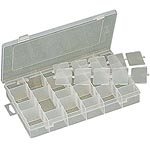
\includegraphics[width=0.45\textwidth]{tech/tools/proskit/103-132D.jpg}
&
\noindent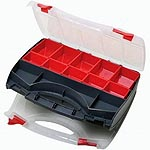
\includegraphics[width=0.45\textwidth]{tech/tools/proskit/SB-3428SB.jpg}
\\
\textbf{103-132D Кассетница для деталей и компонентов}
&
\textbf{SB-3428SB Портативная кассетница для саморезов и т.п.}
\\
\end{tabular}
\clearpage

\secrel{Радиомонтаж}

\begin{tabular}{p{0.45\textwidth} p{0.45\textwidth}}
\noindent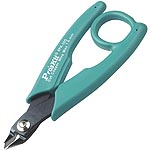
\includegraphics[width=0.45\textwidth]{tech/tools/proskit/8PK-30D.jpg}
&
\noindent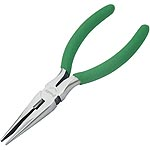
\includegraphics[width=0.45\textwidth]{tech/tools/proskit/1PK-709.jpg}
\\
\textbf{8PK-30D Кусачки миниатюрные}
&
\textbf{1PK-709 Длинногубцы-кусачки}
\\
\end{tabular}
\clearpage

\begin{tabular}{p{0.45\textwidth} p{0.45\textwidth}}
\noindent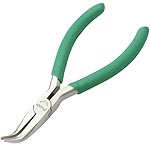
\includegraphics[width=0.45\textwidth]{tech/tools/proskit/1PK-055S.jpg}
&
\noindent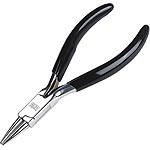
\includegraphics[width=0.45\textwidth]{tech/tools/proskit/1PK-29.jpg}
\\
\textbf{1PK-055S Длинногубцы изогнутые}
&
\textbf{1PK-29 Круглогубцы}
\\
\end{tabular}
\clearpage

\begin{tabular}{p{0.45\textwidth} p{0.45\textwidth}}
\noindent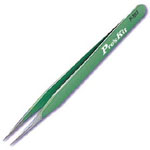
\includegraphics[width=0.45\textwidth]{tech/tools/proskit/1PK-101T.jpg}
&
\noindent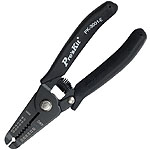
\includegraphics[width=0.45\textwidth]{tech/tools/proskit/1PK-3001E.jpg}
\\
\textbf{1PK-101T Пинцет прямой}
&
\textbf{1PK-3001E Клещи для зачистки проводов прецизионные (стриппер)}
\\
\end{tabular}
\clearpage

\begin{tabular}{p{0.45\textwidth} p{0.45\textwidth}}
\noindent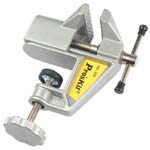
\includegraphics[width=0.45\textwidth]{tech/tools/proskit/PD-374.jpg}
&\\
\textbf{PD-374 Тиски на струбцине}
&\\
\end{tabular}
\clearpage

\secrel{Прочие}

Попалась интересная недорогая отвертка: aиксация четкая, исполнение очень
неплохое, позволяет добраться до узких мест. Из минусов: ручка похоже не
цельнометаллическая, при изломе есть риск распороть руку.

\bigskip
\noindent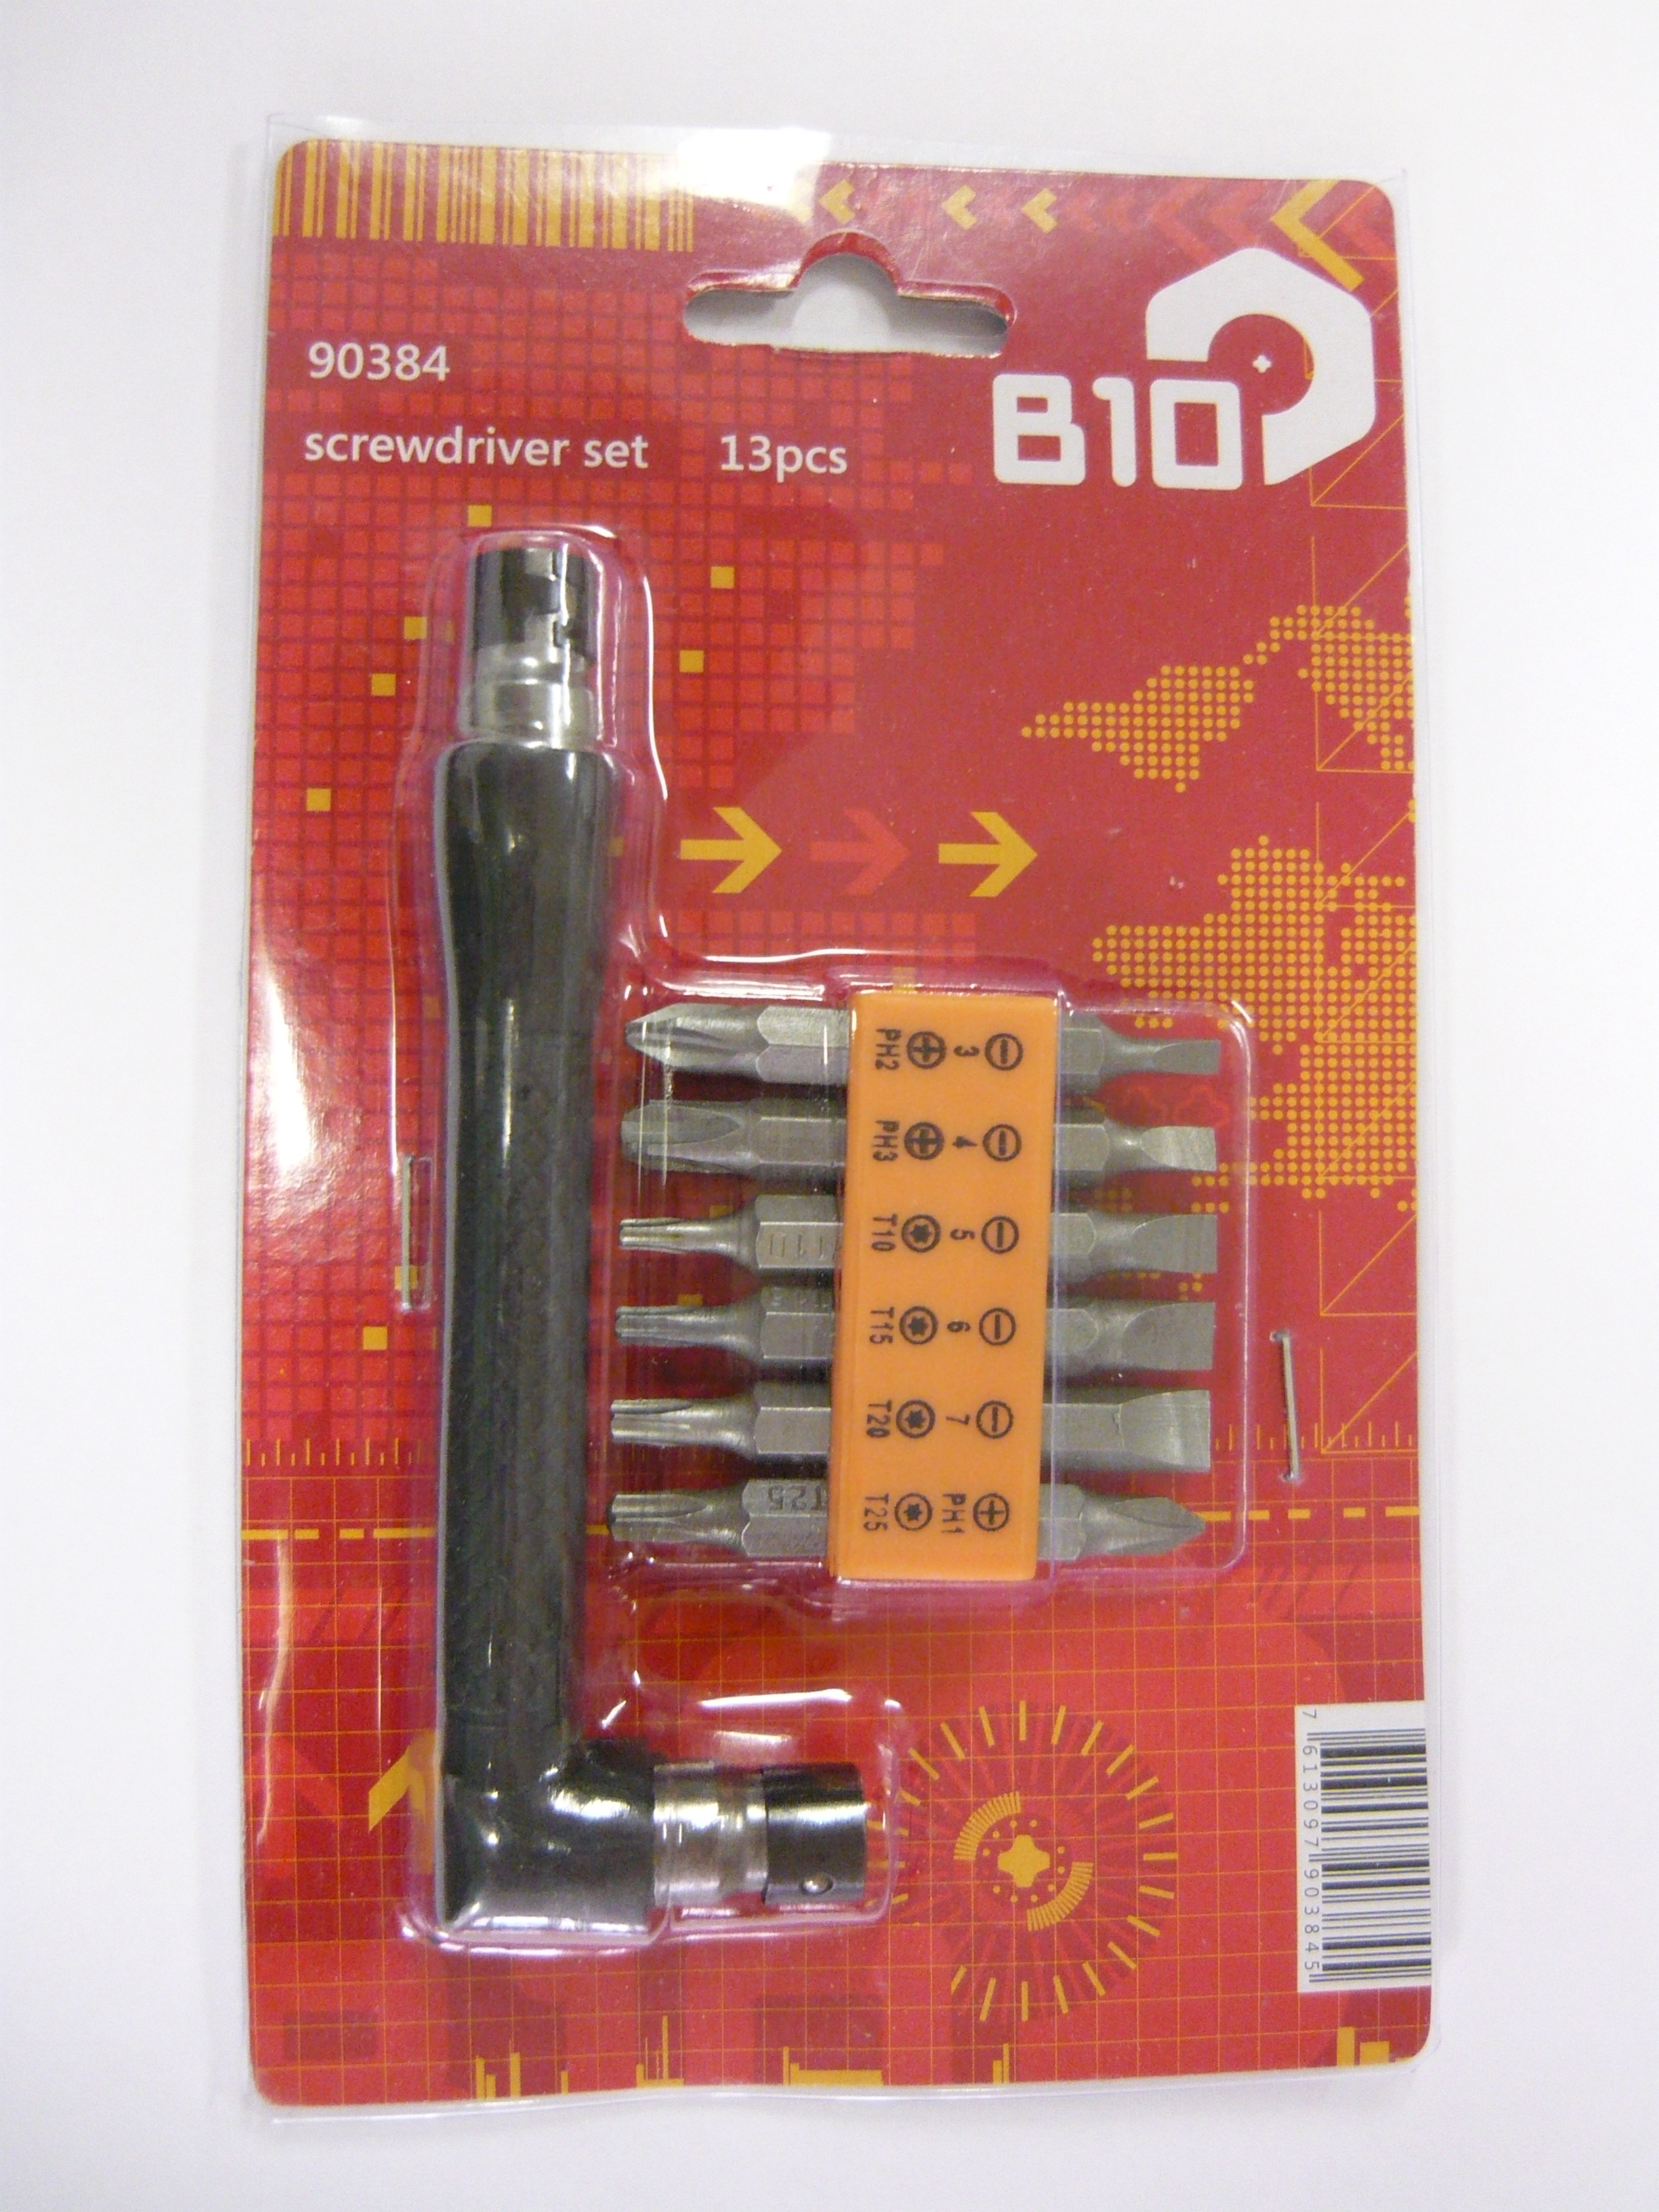
\includegraphics[width=0.4\textwidth]{tech/tools/P1020966.jpg}
\noindent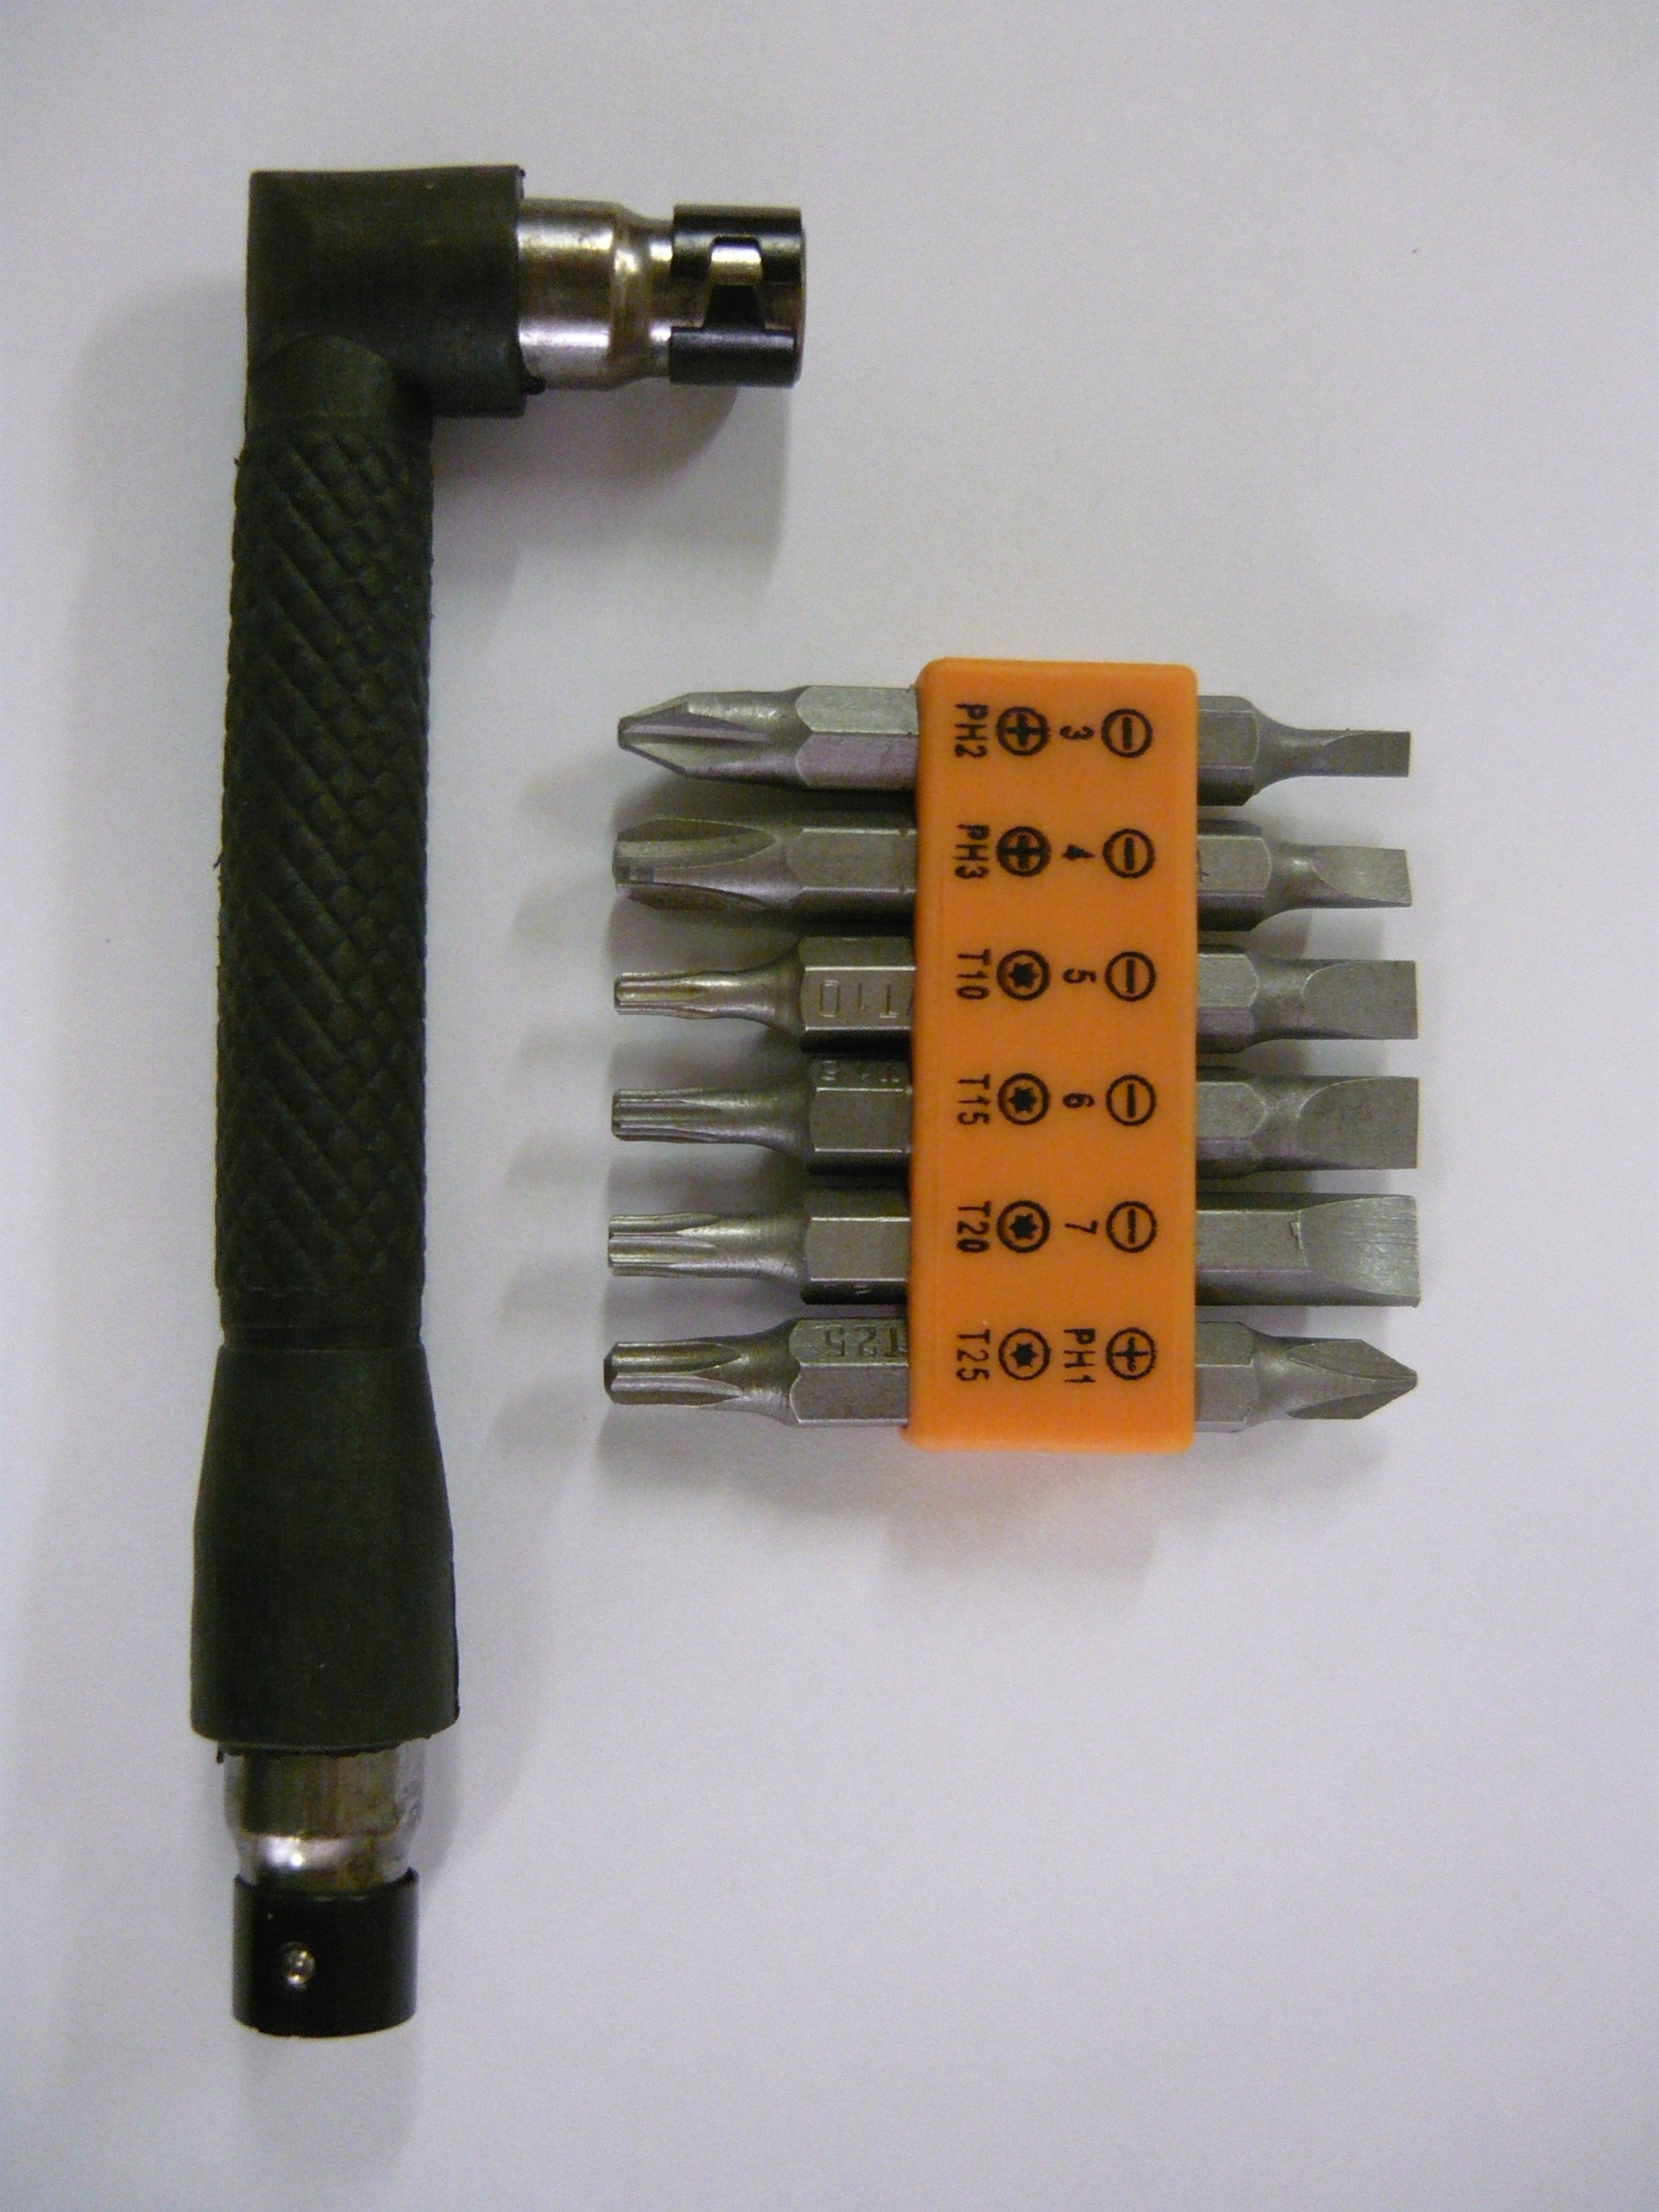
\includegraphics[width=0.4\textwidth]{tech/tools/P1020967.jpg}
\clearpage

\secup



\section{Измерительное оборудование}

\subsection{Тестер}

\subsection{Осциллограф}

\subsection{Логический анализатор}

\subsection{Генератор сигналов}

\subsection{Рыльцеметр}

\secrel{Электроинструмент}\secdown

\secrel{Дрелъ}

% \noindent
% \begin{tabular}{p{0.5\textwidth} p{0.5\textwidth}}
% \noindent
% 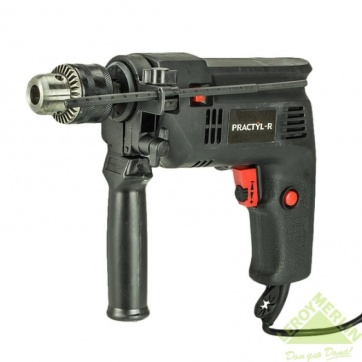
\includegraphics[width=0.45\textwidth]{tech/tools/PraktylR.jpg}
% &
% \noindent
% 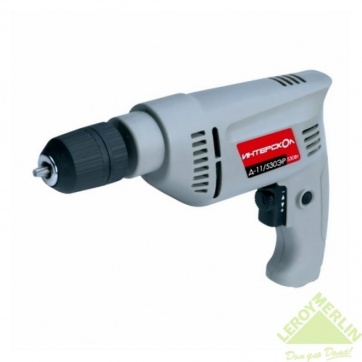
\includegraphics[width=0.45\textwidth]{tech/tools/D_11_530ER.jpg}
% \\
% \textbf{Дрель ударная сетевая} & \textbf{Дрель безударная сетевая} \\
% \textbf{Praktyl-R PID13D01 400\,Вт} 
% \href{http://leroymerlin.ru/catalogue/instrumenty/elektroinstrument/dreli\_udarnye/13805983/}{\textbf{(!)395\,р.}}
% &
% \textbf{Интерскол Д-11/530ЭР (с БЗП)}
% \href{http://leroymerlin.ru/catalogue/instrumenty/elektroinstrument/dreli\_bezudarnye/11857763/}{\textbf{1120\,р.}}
% \\
% \end{tabular}
% \bigskip
% 
% Дрель\ --- одноразовая китайчатина от 400\,р. Продаются уже брендированные на
% Леруа Мерлен, наклейка <<PID13D01 Ударная дрель 400\,Вт, 13\,мм>>. Скорость
% регулируется глубиной нажатия курка, крутилка на курке ограничивает глубину
% механически, фиксатор держит скорость близко к минимальной, запаха горелой
% пластмассы через несколько минут работы на холостом ходу нет.
% 
% По надежности рекомедуется Интерскол 1100+\,р. Надежность Интерскола\ --- не
% <<китай>>, классика ДУ-580ЭР работает в хвост и гриву, используется криворукими
% студентами, лежит в подвале в пыли от точила, и никаких вопросов даже со
% щетками.
% 
% Если не планируете много сверлить бетон, \textbf{берите дрель без ударного
% механизма}: отсутствуют лишние продольные перемещения, что может быть важно при
% использовании в качестве шпинделя сверлильного станка, и механизации других
% технологических поделок.
% 
% У шуруповерта нет 43\,мм шейки для фиксации, поэтому как средство электропривода
% он практически бесполезен, и нужен собственно для заворачивания большого
% количества саморезов. Хотя наличие ограничителя крутящего момента и малые
% габариты удобны при сверлении и сборке поделок.
% 
% \bigskip
% Имея некоторое количество поделочного материала, кривые руки и особенно доступ к
% станочному оборудованию, можно сколкозить некоторое подобие настольных
% станочков\ \pref{fig:drelstans}\ для механизации некоторых работ,
% используя дрель в качестве привода.
% 
% Главным элементом такой оснастки\ --- зажим на шейку дрели 43\,мм. Особых
% требований по его точности и качеству нет, т.к. сама шейка обычно пластиковая, и
% никакой доводки по круглости и параллельности оси инструмента не проходит.
% 
% \clearpage
% \phantomsection\label{fig:drelstans}
% \noindent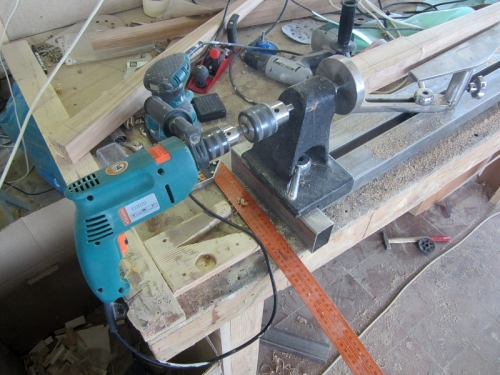
\includegraphics[height=0.528\textheight]{tech/tools/DrelLathe.jpg}
% \noindent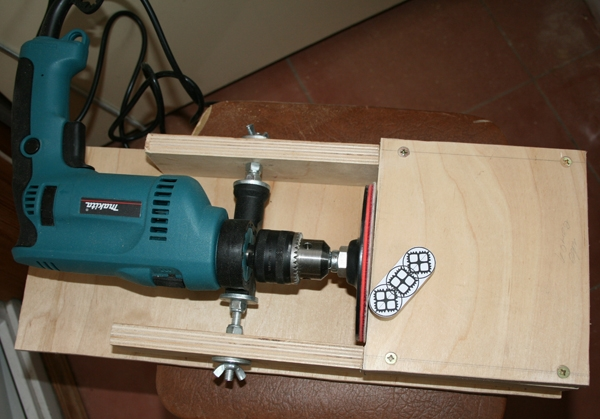
\includegraphics[height=0.528\textheight]{tech/tools/DrelShliph.jpg}
% 
% \noindent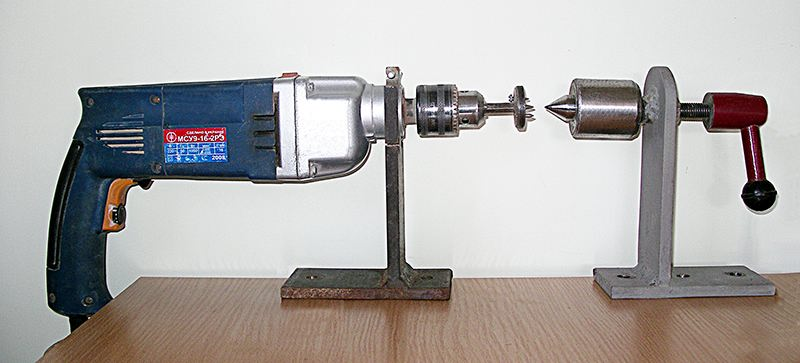
\includegraphics[height=0.465\textheight]{tech/tools/DrelLathe2.jpg}
% \noindent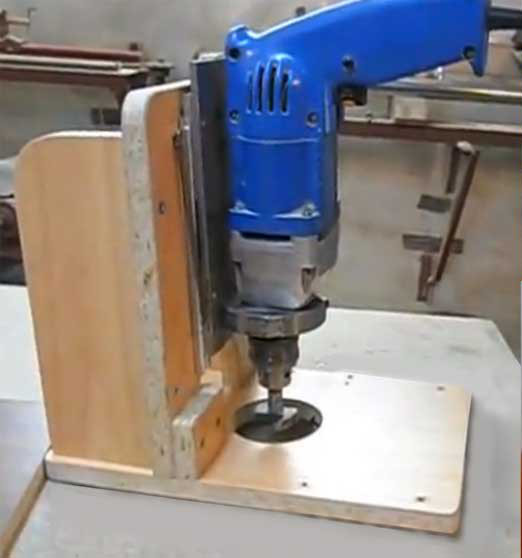
\includegraphics[height=0.465\textheight]{tech/tools/DrelBoren.jpg}
% \clearpage

\secrel{Лобзик}

% \noindent
% \begin{tabular}{p{0.5\textwidth} p{0.5\textwidth}}
% \noindent
% 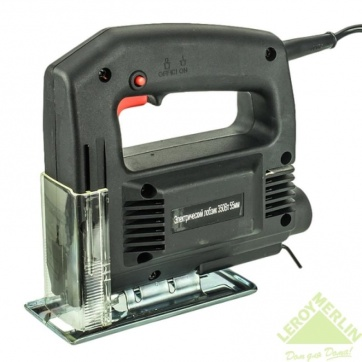
\includegraphics[width=0.45\textwidth]{tech/tools/LobzPraktyl.jpg}
% &
% \noindent
% 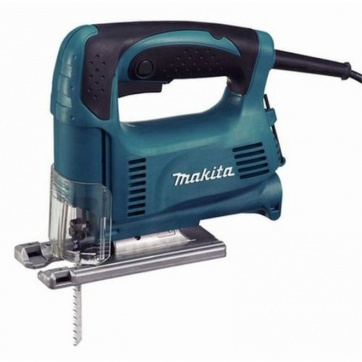
\includegraphics[width=0.45\textwidth]{tech/tools/LobzMakita4329.jpg}
% \\
% \href{http://leroymerlin.ru/catalogue/instrumenty/elektroinstrument/lobziki/13805991/}{\textbf{Praktyl
% 350 Вт 356\,р.}} 
% & 
% \href{http://leroymerlin.ru/catalogue/instrumenty/elektroinstrument/lobziki/12114283/}{\textbf{Makita
% 4329 2260\,р.}}
% \\
% \end{tabular}
% \bigskip
% 
% Лобзик полезен при разделке стеклотекстолита, и изготовлении технологической
% мебели (стеллажи, рабочие столы и т.п.).

\secrel{Жвигатель}

% Если у вас возникло желание механизировать изготовление механических деталей, а
% свободного доступа к настоящему станочному оборудованию нет, есть смысл
% рассмотреть изготовление самодельной механизированной оснастки 
% типа\ \pref{fig:drelstans}, или даже самодельных станочков. В этом случае надо
% рассмотреть применения универсального привода.
% 
% Первый кандидат на место универсального электропривода достается той самой
% дрели, не забываем об обязательном наличии 43\,мм монтажной шейки.
% Достоинство дрели как привода\ --- прямое подключение к сети, встроенный
% редуктор, есть модели с простой регулировкой оборотов, есть резьба и отверстие
% под винт на валу, в комплекте есть патрон для зажима мелких деталей в
% точилке\footnote{\ БЗП удобен, патрон с ключем дает лучший зажим и возможно
% точнее}.
% 
% Ограниченно доставаемые двигатели от стиральных машин, отличаются мощностю и
% оборотистостью, особенно от старых моделей. Часто доступны сразу с готовым
% шкивом на валу, который иногда проще использовать, чем снять.
% 
% Автозапчасти: привод печки Камаза, двигатель постоянного тока 
% 24\,В 50\,Вт
% 
% Новые асинхронные двигатели АИРЕ 56 B2/B4 (3000/1500 об.) с заводским
% конденсатором, подключается к сети $\sim$220\,В, цена от 2500\,р.
% С ростом размеров и мощности цена резко повышается.
% Следует обратить внимание на возможность монтажа на дополнительный фланцевый
% подшипниковый щит, (?) с моделями АИРЕ 80.
% 
% Для самодельных серлилок и микроинструмента хороши китайские воздушные шпиндели
% постоянного тока с цанговыми патронами ER11. Требуют источник питания
% постоянного тока 9$\div$48\,В. В магазинах не попадались, необходима прямая
% покупка с \href{http://www.aliexpress.com/}{AliExpress}\note{пользуйтесь
% английской версией\ --- переводная жуткое УГ}\ по почте.
% 
% % \clearpage
% \begin{tabular}{l l}
% 
% \noindent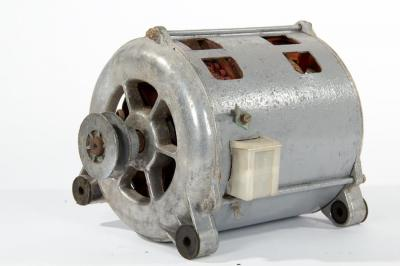
\includegraphics[width=0.37\textwidth]{tech/tools/VyatkaDvig.jpg} 
% & 
% \noindent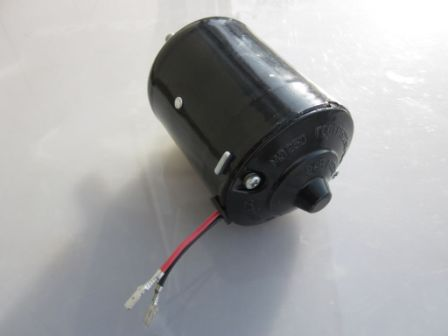
\includegraphics[width=0.37\textwidth]{tech/tools/KamazDvig.jpg}
% \\
% \textbf{Жвигатель Вятка-Автомат 19??\,г.}
% &
% \textbf{Двигатель печки Камаза}
% \\
% 
% \noindent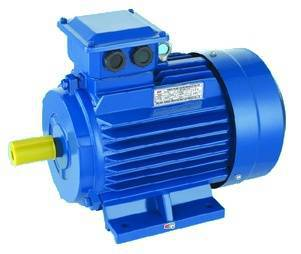
\includegraphics[width=0.37\textwidth]{tech/tools/AIRE.jpg}
% & 
% \noindent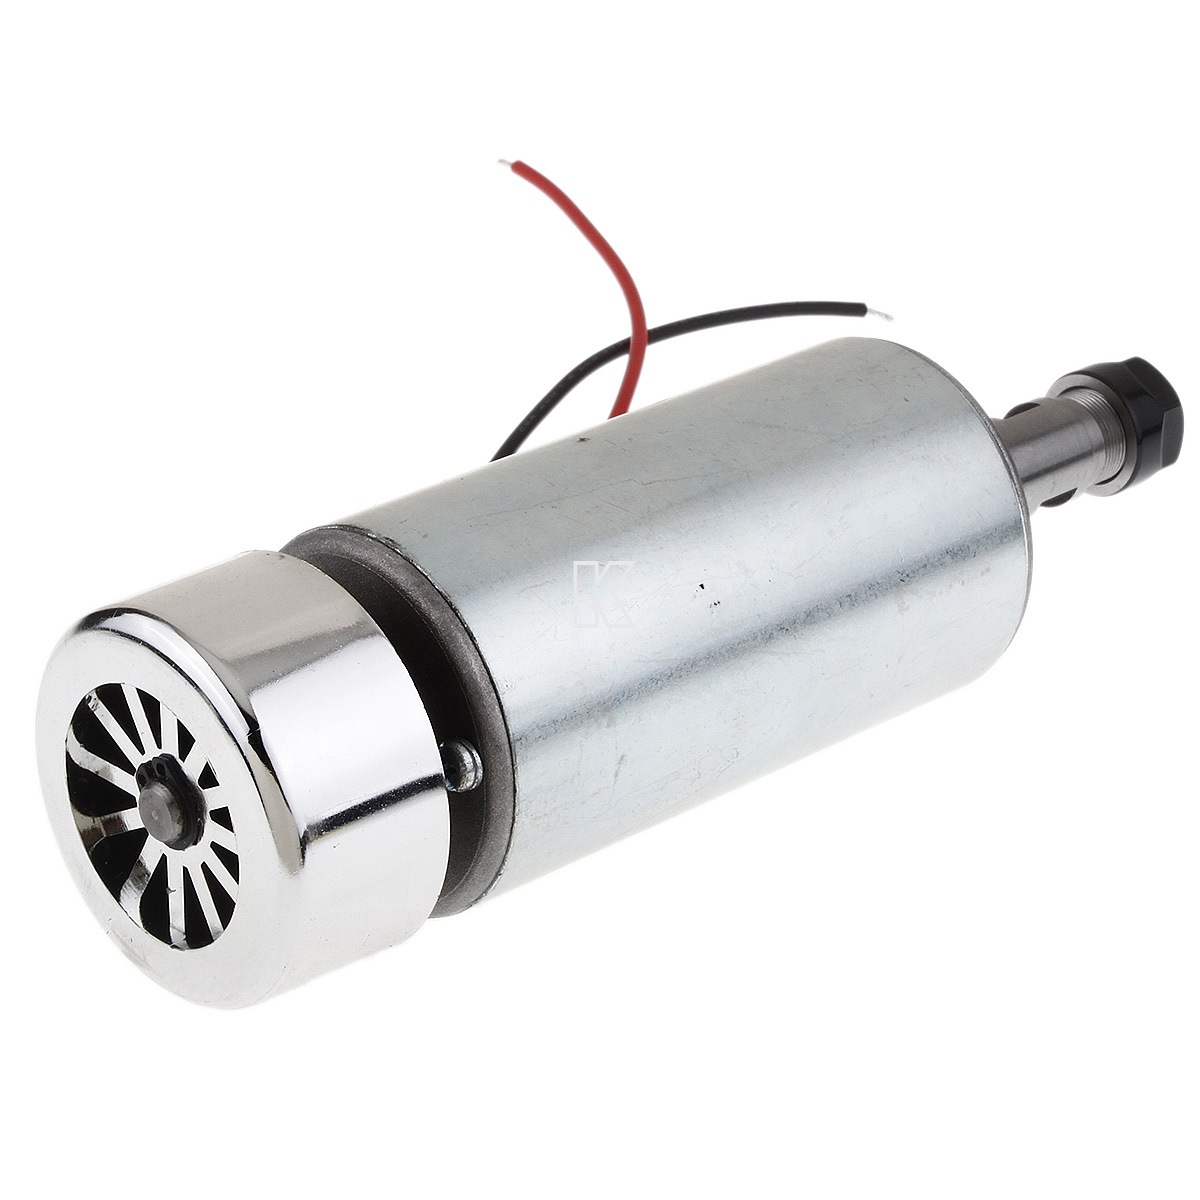
\includegraphics[width=0.37\textwidth]{tech/tools/ER11.jpg}
% \\
% \textbf{АИРЕ 56 B2, 0.2\,КВт}
% &
% \textbf{Воздушный шпиндель с цангой ER11}
% \\
% 
% \end{tabular}
% \clearpage
% 
% Съемные фрезерные шпиндели, поставляются отдельно или в комплекте с насадкой
% ручного фрезера по дереву. Лучшие, со стальной шейкой\ --- Kress, активно
% применяются хобби-ЧПУшниками. Попроще и сильно дешевле делал Интерскол, иногда
% попадается noname. Недостаток как универсального привода\ --- они
% высокоскоростные, возникают проблемы с понижающими передачами. Применение\ ---
% приводной высокоскоростной инструмент: боры, фрезы по дереву, микроинструмент
% для граверов (микродиски, шарошки). Цанга 8\,мм. Для некоторых моделей бывают
% наборы цанг на мелкий инструмент.
% 
% \bigskip
% \begin{tabular}{p{0.3\textwidth} p{0.3\textwidth} p{0.3\textwidth} }
% \noindent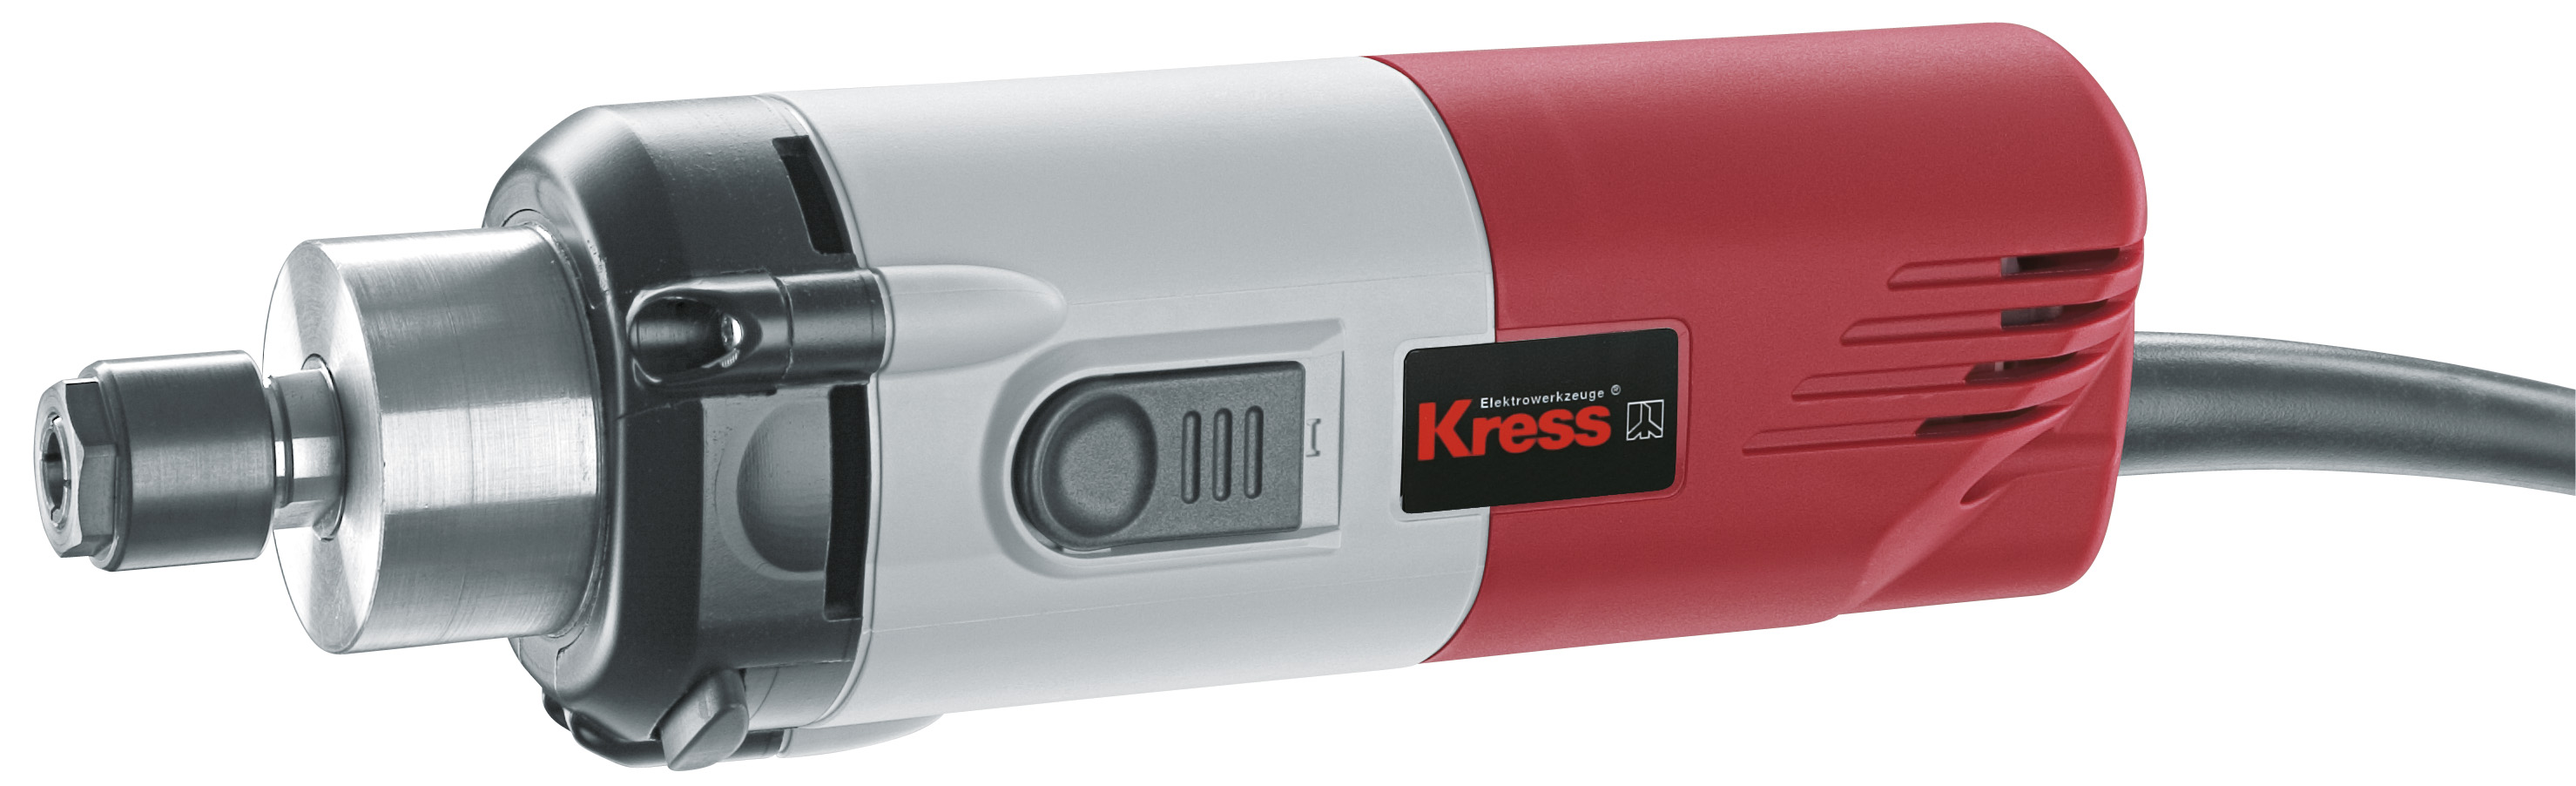
\includegraphics[height=0.3\textheight,width=0.3\textwidth,keepaspectratio]{tech/tools/Kress530.jpg}
% &
% \noindent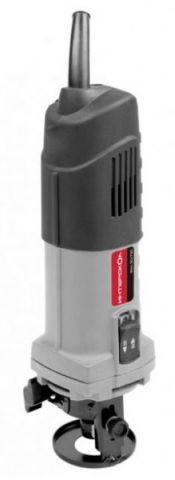
\includegraphics[height=0.3\textheight,width=0.3\textwidth,keepaspectratio]{tech/tools/Interskol30.jpg}
% &
% \noindent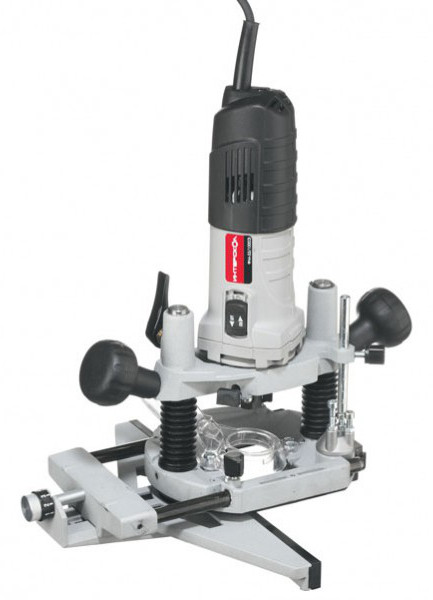
\includegraphics[height=0.3\textheight,width=0.3\textwidth,keepaspectratio]{tech/tools/InterskolFM55.jpg}
% \\
% KRESS 530/800/1050 FM(E)
% &
% Интерскол ФМ-30/750
% &
% Интерскол ФМ-55/1000 Э
% \\
% \href{http://kress-shop.ru/product/frezernyj-dvigatel-530-fm-kress-06082302/}{5600+\,р.}
% &
% /снят с производства/
% &
% \href{http://www.kuvalda.ru/catalog/1867/27920/}{5050\,р.}
% \\
% \end{tabular}

\secup


